\chapter{Step Size Adaptation}
\label{ch: stepsize_adaptation}

\graphicspath{{Figures/Stepsize_adapt/}{./}} 

\section{Failure on Newton's Method}
\label{sec: newton}
Newton's method is an iterative method to find the stationary points (where the function's derivative is zero) of a twice-differentiable function $f$. The application of Newton's method failed for our SGD quantile methods, since the loss function of the quantile estimation function is not twice-differentiable. For a specific $\tau$, and $t := x - q$ be the difference between the input data value $x$ and the estimate of quantile $q$, the loss function 

\begin{equation}
    \ell_\tau(t)= 
        \begin{cases}
            \tau t & t > 0\\
            -(1-\tau) t & otherwise
        \end{cases}
\end{equation}


is a linear function of $t$, which doesn't have any second derivative. 
\\\\
Though the method cannot be applied, it is easy to reach the goal of Newton's method: to find the critical points of a function. Instead of stationary point, the loss function has a critical point where it is not differentiable and the derivative changes sign. For any $\tau \in (0,1)$, when $t=0$, the loss function reaches it's critical points at $\ell_\tau(0) = 0$. Taking the critical point for every step, however, does not contribute to any improvement in quantile estimation. To be at a critical point, the quantile estimate is set to have the equal value of input data $x$, and only in this way we could have $t = x-q = x-x = 0$. Regardless of $\tau$, the quantile estimate is always equal to the value of the latest data point. So far this method has totally failed its goal to estimate a quantile value based on $\tau$ and the entire data stream.
\\\\
From another perspective, the failure of Newton's method is the result of applying large step size for the last input data for a SGD method. In this way, the minimal of current loss function $\ell_\tau(t)$ is reached, while the total loss function for the input data stream $X$

\begin{equation}
    L_{\tau}(t) = \sum_{x \in X} \ell_{\tau}(t)
\end{equation}

is entirely ignored.

% ------------------------------------------------

\graphicspath{{Figures/Smooth_func/}{./}} 


\section{Stochastic Average Gradient (SAG)}
\label{sec: sag}
One approach on step size adaptation is to use the stochastic average gradient (SAG)\cite{schmidtMinimizingFiniteSums2016} algorithm. It is an convex optimization method that has a significant improvement of convergence rate than stochastic gradient (SG) methods. In general, the convergence rate is improved from $O(1/\sqrt{k})$ to $O(1/k)$ for a total of $k$ epochs, reaching the same level as the gradient descent method. Along with the rising convergence rate, it keeps a low computational cost for each iteration to be independent from the size of function sum.

\subsection{Mechanism of SAG}
Similar to SG methods, SAG methods aim for minimization of the sum of a finite number of smooth convex functions where $N$ is very large. The problem setting is
\begin{equation}
\underset{x \in \mathbb{R}^p}{\text{minimize}} g(x) := \frac{1}{N}\sum^N_{n=1} \ell_n(x)
\end{equation}
where each $\ell_n$ is a smooth convex function.

The standard (full) gradient (FG) method has each iteration in the form
\begin{equation}
x_{i+1} = x_i - \alpha_i g^{\prime} (x_i) = x_i - \frac{\alpha_i}{N}\sum^N_{n=1} \ell_n^{\prime}(x_i)
\end{equation}
where $\alpha_i$ is the step size of iteration $i$. For each iteration, the computational cost is $O(N)$.

To save the iteration cost, the stochastic gradient (SG) method has each iteration in the form
\begin{equation}
x_{i+1} = x_i - \alpha_i \ell_{m_i}^{\prime} (x_i)
\end{equation}
where $m_i$ is the index for the iteration that gets sampled from the range {$1, 2,...,n$}. It has an iteration cost of $O(1)$, but a much lower convergence rate.

The stochastic average gradient (SAG) remembers the last update of a gradient value for each index $i$, which enables the improvement of convergence rate from SG methods. Its iteration takes the form
\begin{equation}
x_{i+1} = x_i - \frac{\alpha_i}{N} \sum^N_{n=1}y_{m}^{i}
\end{equation}
where $y_{m}^{i}$ is used to keep the memory of recently updated gradient value of function $\ell_m$
\begin{equation}
y_{m}^{i}:=\left\{\begin{array}{ll}
    \ell_{m}^{\prime}\left(x_{i}\right) & \text { if } m=m_{i} \\
    y_{m}^{i-1} & \text { otherwise }
    \end{array}\right.
\end{equation}
The SAG algorithm, according to \citeauthor{schmidtMinimizingFiniteSums2016}, "like the FG method, the step incorporates a gradient with respect to each function". Meanwhile only one gradient computation is involved in the combination of gradients, such that the iteration cost is independent of $N$.

\subsubsection{Convergence guarantee}

Under the assumption that each $\ell_m$ is convex and the gradient $\ell_m\prime$ is \textit{Lipschitz continuous} with constant $L$, which means
\begin{equation}
|\ell_m\prime (a) - \ell_m\prime (b)| \leq L|a-b|
\end{equation}
for all $a,b \in \mathbb{R}^p$.
The SAG algorithm with constant step size $\alpha_i = \frac{1}{16L}$ reaches the convergence rate of $O(1/i)$. The convergence function differs when the $y_m^0$ is initialized differently, or when $l_m$ is strongly convex.


\subsection{Basic SAG algorithm}

\begin{algorithm}
    \caption{Basic SAG method for minimizing $\frac{1}{N} \sum^N_{n=1}\ell_n(x)$ with step size $\alpha$}\label{alg:SAG_ori}
        \begin{algorithmic}[1]
            \Require{Dataset $X$, Dataset Size $N$, Step size $\alpha$}
            \Ensure{$x$}
            % \Procedure{frugal}{$X,\tau$}            \Comment{X is the dataset}
            \State {$d = 0, y_m = 0$ for $m = 1, 2, ..., N$}           \Comment{Default initialization}
            \For{$i = 0,1,...$}                  %\Comment{Parameter update for each input data point}
                \State {Sample $m$ from $\{1,2,...,N\}$}
                \State {$d=d - y_m + \ell^{\prime}_m(x)$}
                \State {$y_m = \ell^{\prime}_m(x)$}                    \Comment{Save the $y_m$ in the table for re-visit}
                \State{$x = x - \frac{\alpha}{N}d$}
            \EndFor
            \State{\textbf{end for}}
        \end{algorithmic}
\end{algorithm}

The Basic SAG algorithm requires memory storage of a table of $y_m (m= 1, 2, ...,N)$, to keep the track of each $y_m$ in case they are re-visited after first update.

\subsection{SAG Implementation for quantile estimation}

The quantile estimation loss function is a convex function, and \textbf{we can use a smooth function for replacement}
\begin{algorithm}
    \caption{Basic SAG method for streaming data $S$ for quantile estimation}\label{alg:SAG}
        \begin{algorithmic}[1]
            \Require{Data Stream $X$, Data Stream Size $N$, $\tau$, $\tau$-quantile estimate $\tilde{q}$, Step size $\alpha$}
            \Ensure{$\tilde{q}$}
            % \Procedure{frugal}{$X,\tau$}            \Comment{X is the dataset}
            \State {Initialization $d = 0, \tilde{q}=0$}           \Comment{Default initialization $q_0=0$, $d_0=0$}
            \For{\textbf{each} $x_i$ in $X$}                  %\Comment{Parameter update for each input data point}
                \State {$d=d - 0 + \ell^{\prime}_{\tau}(x_i, \tilde{q})$} \Comment{$0$ stands for $y_m^{i-1}$}
                % \State {\textbf{set} $\alpha_k$} \Comment{Set stepsize}
                \State{$\tilde{q} = \tilde{q} - \frac{\alpha}{N}d$}
            \EndFor
            \State{\textbf{end for}}
        \end{algorithmic}
\end{algorithm}
For streaming data, it's worthwhile noticing that each input data point has exactly one pass. It means for the SAG implementation, the storage of updated $y_m^i$ is useless since it would not be revisited. Besides, if all $y_m^0$ are initialized as 0, the storage of $y^0$ initialization needs only one unit of memory instead of $N$ units of memory. in this way, we can keep the memory complexity of SAG quantile estimation to $O(1)$.

\subsection{Experiments on SAG}

In this section, we explore how SAG

\graphicspath{{Figures/Stepsize_adapt/SAG/}{./}} 

\begin{figure}[H]
    \centering
	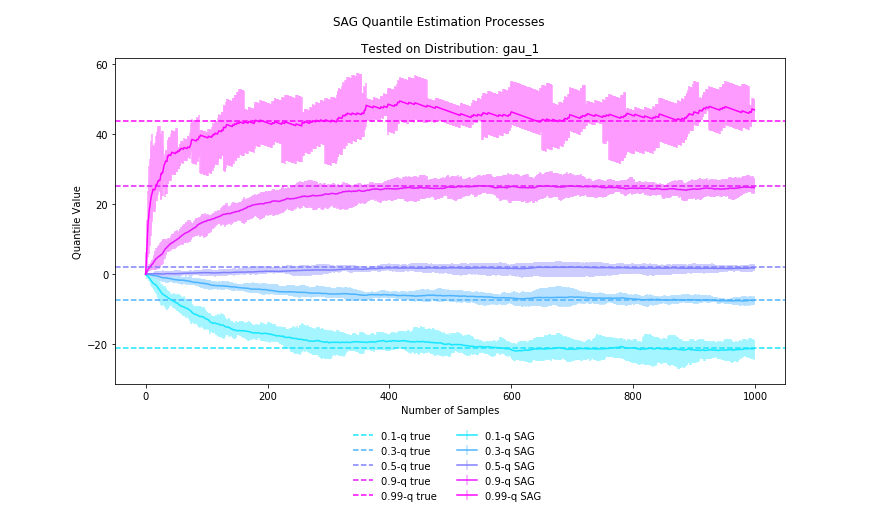
\includegraphics[width=1\columnwidth]{distro/gau_1_proc.png}
	\caption{SAG Process from \textit{gau-1} Distribution}
\end{figure}

\begin{figure}[H]
    \centering
	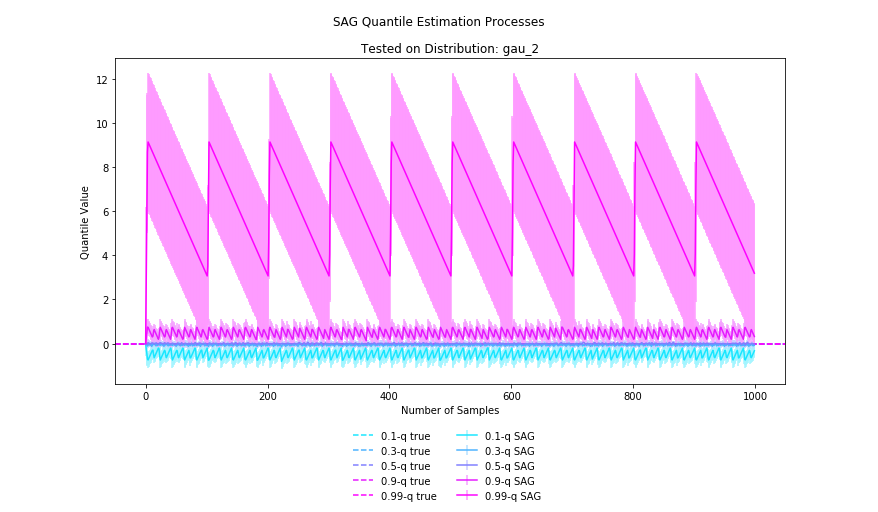
\includegraphics[width=1\columnwidth]{distro/gau_2_proc.png}
	\caption{SAG Process from  \textit{gau-2} Distribution}
\end{figure}

\begin{figure}[H]
    \centering
	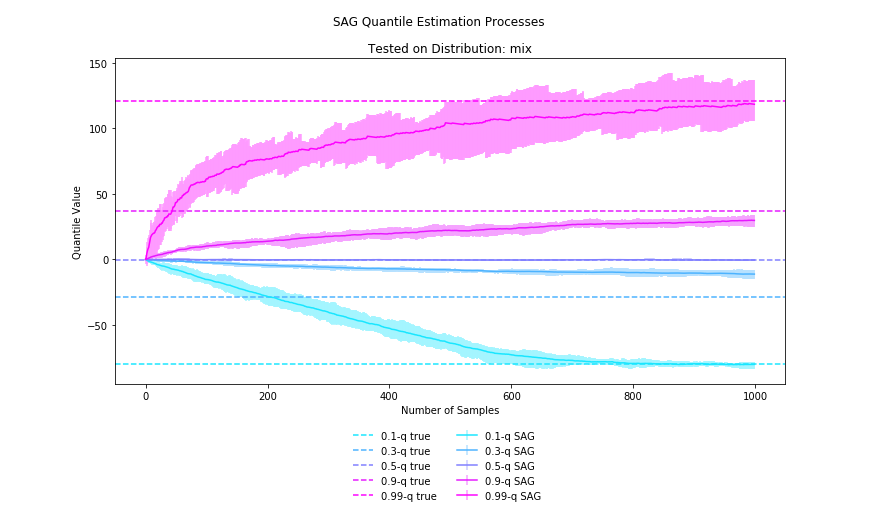
\includegraphics[width=1\columnwidth]{distro/mix_proc.png}
	\caption{SAG Process from \textit{mix} Distribution}
\end{figure}

\begin{figure}[H]
    \centering
	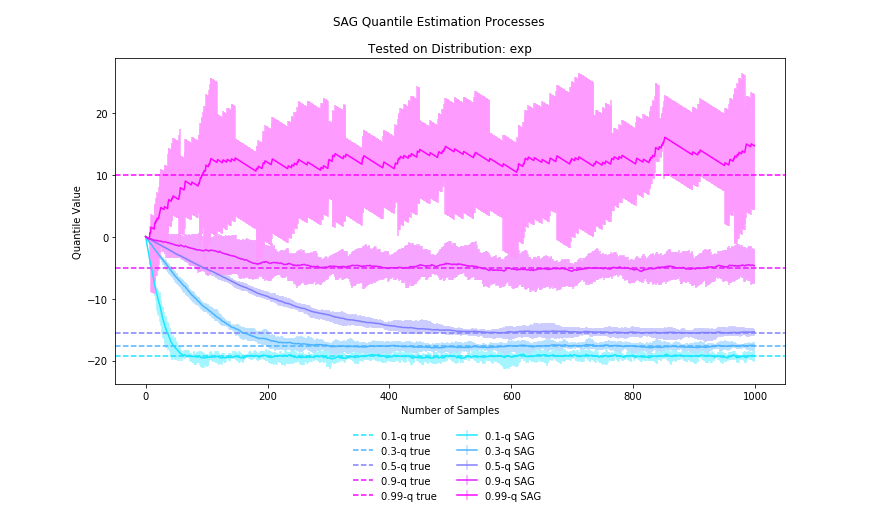
\includegraphics[width=1\columnwidth]{distro/exp_proc.png}
	\caption{SAG Process from \textit{exp} Distribution}
\end{figure}

\begin{figure}[H]
    \centering
	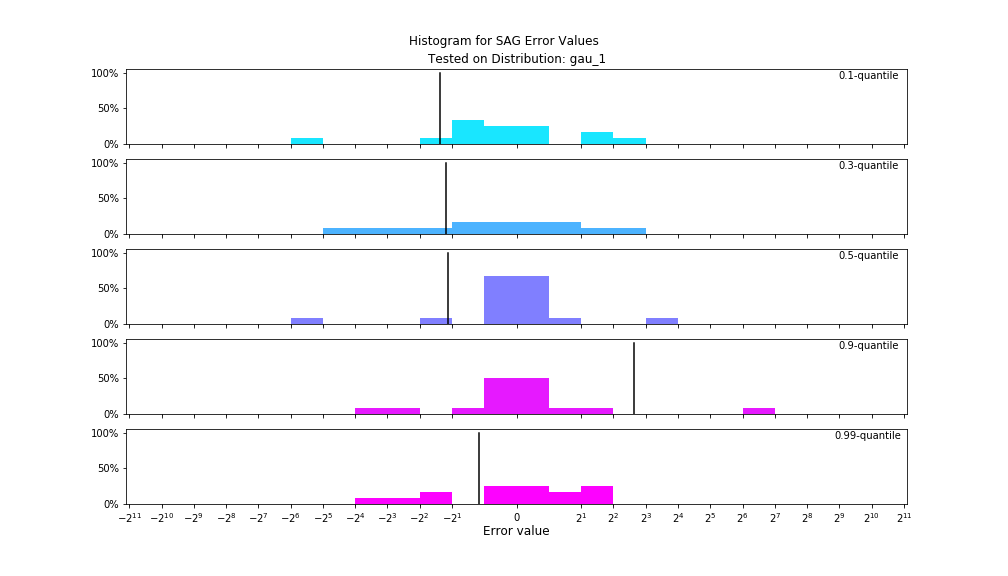
\includegraphics[width=1\columnwidth]{distro/gau_1_err.png}
	\caption{SAG Error from \textit{gau-1} Distribution}
\end{figure}

\begin{figure}[H]
    \centering
	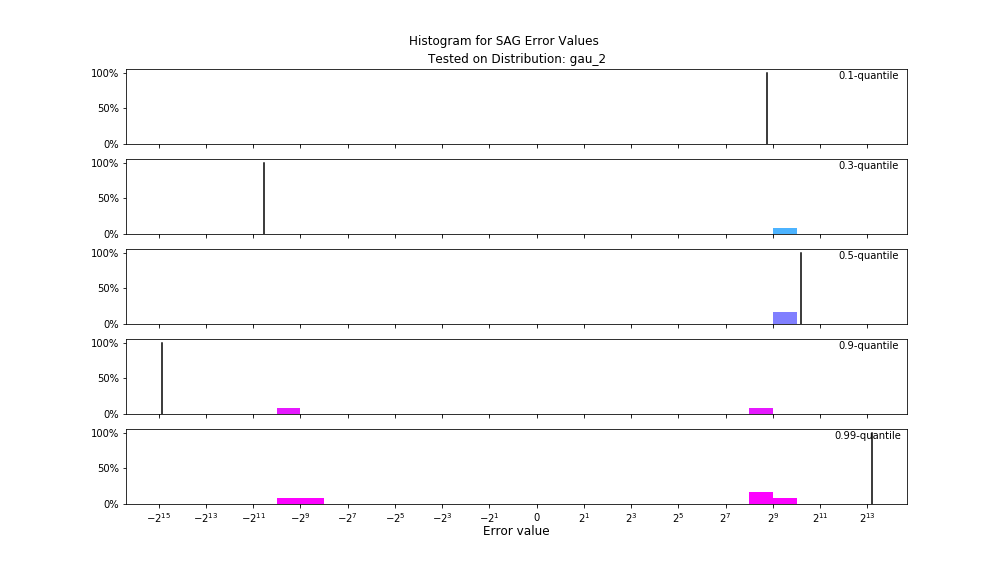
\includegraphics[width=1\columnwidth]{distro/gau_2_err.png}
	\caption{SAG Error from  \textit{gau-2} Distribution}
\end{figure}

\begin{figure}[H]
    \centering
	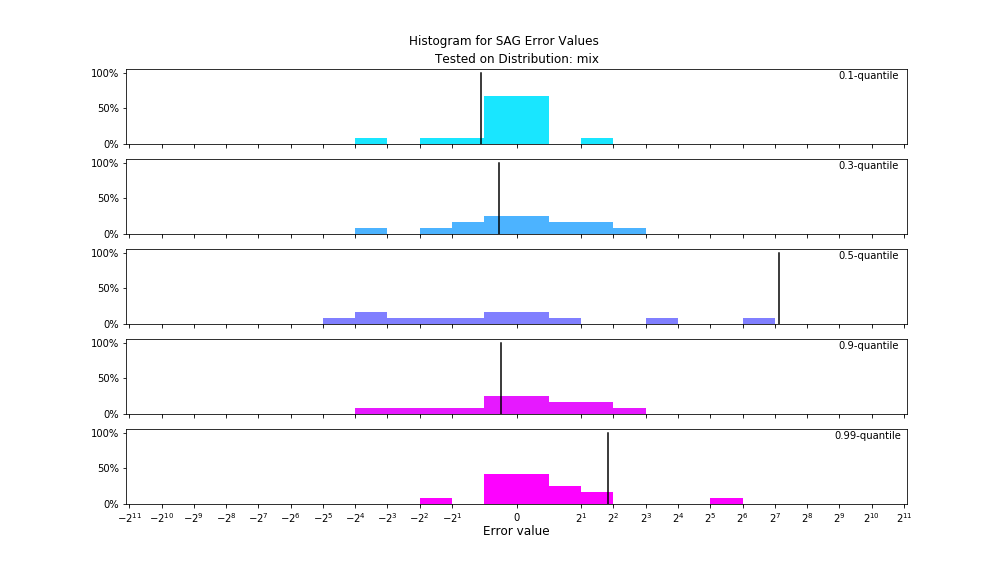
\includegraphics[width=1\columnwidth]{distro/mix_err.png}
	\caption{SAG Error from \textit{mix} Distribution}
\end{figure}

\begin{figure}[H]
    \centering
	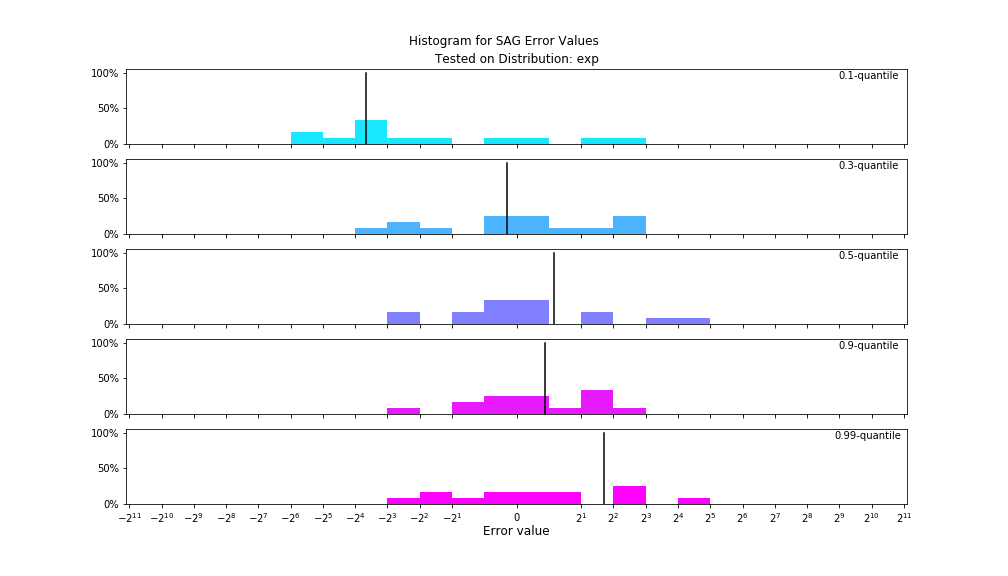
\includegraphics[width=1\columnwidth]{distro/exp_err.png}
	\caption{SAG Error from \textit{exp} Distribution}
\end{figure}

\subsection{Smooth Functions}
The pinball loss function we use for the SGD quantile estimation is convex but not smooth. 
Theoretically, however, both SGD and SAG methods need smoothness for the guarantee of convergence. Although the practical experiments have shown that there is evidence of convergence in final performance, it remains a serious problem for our SGD quantile estimation methods. In this section, we present the analysis on the non-smoothness problem, followed by the potential solutions and further discussions on them.

\subsubsection{The Pinball Loss Functions}
\graphicspath{{Figures/Stepsize_adapt/Smooth_func/}{./}} 

The pinball loss function evaluates the loss from a data point $x$ for estimation of the $\tau$-quantile.

\textbf{quote the equation of pinball loss function and it's derivative}

The fact that the pinball loss function is not differentiable at $x= 0$ has became a problem for the stochastic gradient descent which uses derivatives of object functions.

\begin{figure*}[h!]
	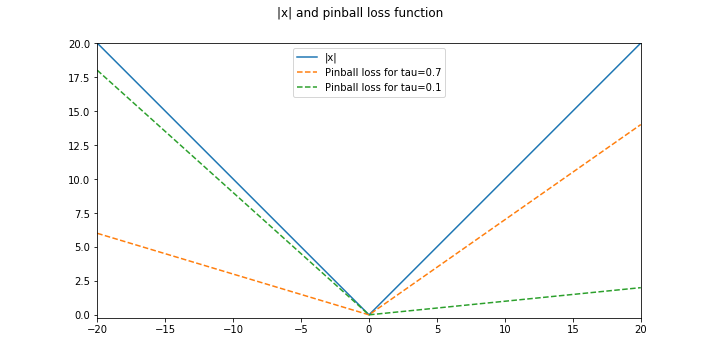
\includegraphics[width=1\columnwidth]{abs_pinball.png}
	\caption{Comparison between $|x|$ and the pinball loss function with different $\tau$ values}
\end{figure*}

The absolute function and the pinball loss function are obviously very much alike. In fact, with simple manipulation, the pinball loss function can be written in the form of absolute function as 
\begin{equation}
    l_\tau(x) = 
    \begin{cases}
        \tau \cdot |x| & {x \geq 0} \\
        (1-\tau) \cdot |x| & \text{otherwise}
    \end{cases}
\end{equation}
The pinball loss function is the combination of $|x|$ on the two parts $x<0$ and $x>0$ with different constant scale. 
If the derivative of the smooth function for $|x|$ at $x=0$ is $0$, we can also use the same approximation function respectively for the two parts of the pinball loss.
\\\\
In section \ref{subsec: smooth_sqrt} and \ref{subsec: smooth_new}, we show two approximation functions with regards to the absolute function $f = |x|$, along with the application of the approximations on the pinball loss function.

\subsubsection{Smooth function 1: a simple approxitmation}
\label{subsec: smooth_sqrt}

For $f = |x|$, a common and simple smooth approximation is $
    f = \sqrt{x^2 + \mu^2}
$.
 The convergence towards the absolute function is then proved by \citeauthor{voroninConvolutionBasedSmooth2015a}\cite{voroninConvolutionBasedSmooth2015a} that 
\begin{equation}
    ||x| - \sqrt{x^2 + \mu^2}| \leq \mu \text{  where } \mu > 0 \in \mathbb{R}
\end{equation}
\\
The smooth function application on the pinball loss function is:
\begin{equation}
    l_\tau(x) \approx 
    \begin{cases}
        \tau \cdot \sqrt{x^2 + \mu^2} & {x \geq 0} \\
        (1-\tau) \cdot \sqrt{x^2 + \mu^2} & {x < 0}
    \end{cases}
\end{equation}
and the derivative is
\begin{equation}
    l_\tau\prime(x) \approx 
    \begin{cases}
        \tau \cdot \frac{x}{\sqrt{x^2 + \mu^2}} & {x > 0} \\
        0 & {x=0} \\
        (1-\tau) \cdot \frac{x}{\sqrt{x^2 + \mu^2}} & {x<0}
    \end{cases}
\end{equation}
\subsubsection{Smooth function 2: a transcendental approximation}
\label{subsec: smooth_new}

For a better approximation accuracy, \citeauthor{bagulSMOOTHTRANSCENDENTALAPPROXIMATION2017}\cite{bagulSMOOTHTRANSCENDENTALAPPROXIMATION2017} proposes a new transcendental approximation function 
 \begin{equation}
    g(x) = x \cdot \tanh(x/\mu) \text{  where } \mu > 0 \in \mathbb{R}
 \end{equation}
which also satisfies
\begin{equation}
    ||x| - x \cdot tanh(\frac{x}{\mu})| < \mu
\end{equation}
The derivative of the approximation is
\begin{equation}
    \frac{dg(x)}{dx} = \frac{x}{\mu} \cdot sech^2 (\frac{x}{\mu}) + tanh(\frac{x}{\mu})
\end{equation}
For the pinball loss function, we now have its smooth function in the form:
\begin{equation}
    l_\tau(x) \approx 
    \begin{cases}
        \tau \cdot x \cdot \tanh(x/\mu) & {x\geq 0}\\
        (1-\tau) \cdot x \cdot \tanh(x/\mu) & {x < 0}
    \end{cases}
\end{equation}
and the derivative is
\begin{equation}
\label{eq:smooth_new_d}
    l_\tau\prime(x) \approx 
    \begin{cases}
        \tau \cdot \frac{x}{\mu} \cdot sech^2 (\frac{x}{\mu}) + tanh(\frac{x}{\mu}) & {x\geq 0}\\
        0 & {x=0}\\
        (1-\tau) \cdot \frac{x}{\mu} \cdot sech^2 (\frac{x}{\mu}) + tanh(\frac{x}{\mu}) & {x < 0}
    \end{cases}
\end{equation}
\subsubsection{Discussion and Conclusion}

In this part, we will compare the two alternative smooth functions in the following aspects: computer efficiency, approximation accuracy and
convexity. 
\begin{itemize}
    \item Computation efficiency: \\
    It is proved by \citeauthor{ramirezX2MostComputationally2014}\cite{ramirezX2MostComputationally2014} that $f = \sqrt{x^2 + \mu^2}$ is the most computationally efficient smooth approximation to $|x|$.
    
    On the other hand, we can see from equation \ref{eq:smooth_new_d}, the derivative for $g(x) = x \cdot \tanh(x/\mu)$ is more difficult to compute.
    \item Approximation accuracy: \\
    The following plots show intuitively how fast the two smooth functions approach to $|x|$ for $\mu = 0.01$ and $\mu = 0.001$.
    
    \begin{figure*}[h!]
        \includegraphics[width=1\columnwidth]{{mu_0.001}.png}
        \caption{Comparison between the two smooth functions when $\mu = 0.001$}
    \end{figure*}

    \begin{figure*}[h!]
        \includegraphics[width=1\columnwidth]{{mu_0.0001}.png}
        \caption{Comparison between the two smooth functions when $\mu = 0.0001$}
    \end{figure*}

    We can see $ x \cdot \tanh(x/\mu)$ has a better accuracy.

    \item Convexity\\
    $f = \sqrt{x^2 + \mu^2}$ is convex and  $g(x) = x · \tanh(x/\mu)$ is not.
\end{itemize}

The form of smooth function \textbf{does not really matter for SAG}. It is important to know the existence of Lipschitz continuous smooth function, and then the $L$ of such function must satisfy
\begin{equation}
    L \leq min(|\tau|, |1-\tau|)
\end{equation}
So that no matter which smooth function is used, we can simply take $min(|\tau|, |1-\tau|)$ to compute the step size $\alpha$ for SAG. However, we can still implement those smooth functions for SGD. Further researches can be done on different smooth function implementation on SGD.


\section{Doubling and Halving SGD (DH-SGD)}
\label{sec: DH_SGD}

Although SAG has a faster convergence rate than SGD, it is clear that the fluctuation problem after convergence still exists. Is it possible that a step size adaptation of SGD can minify the fluctuation after the convergence, and at the same time have an improved convergence rate? In this section, we propose a simple algorithm called Doubling and Halving Stochastic Gradient Descent (DH-SGD), which empirically improve those two problems.

\subsection{Method Description}

The idea of the DH-SGD method is trivial - increase the step size if it is too big, and decrease the step size if it is too small. We choose the change of step sizes to be exponential, specifically, increasing it to double size or decrease it to half size. The evaluation of the scale of step size can be vague.  

The psedu-code is shown here

\marginpar{THe step size scaler is different for different quantiles}
\begin{algorithm}
    \caption{DH-SGD algorithm}\label{alg:DH_SGD}
    \begin{algorithmic}[1]
        \Require{Data Stream $X$, $\tau$, $1$ unit of memory $q$, epoch check size $c$}
        \Ensure{$q$}
        % \Procedure{frugal}{$X,\tau$}            \Comment{X is the dataset}
        \State{epochCount $ec = 0$}                       \Comment{The counter for epochs}
        \State{directionCount $dc = 0$}                   \Comment{The accumulation of directions}
        \State{scaler $s = 1$}                    \Comment{The scaler for step size}
        \State {Initialize} $q$                 \Comment{Default initialization $q_0$ = 0}
        \State{}
            \For{$x_i$ in $X$}                  \Comment{Parameter update for each input data point}
                \State{}
                \State{$ec = ec+ 1$}   
                \If{$ec$ \textit{mod} $c = 0$}            \Comment{Change scaler for every $c$ epochs}
                    \If{$|dc| > 0.25c$ }               
                        \State{$s = 2s$}               \Comment{Double $s$ if the update is mostly in one direction}         
                    \Else {\textbf{if} $|dc| < 0.02c$ \textbf{then}}  
                        \State{$s = 0.5s$}             \Comment{Halve $s$ if the update direction barely changes}
                    \EndIf
                
                \EndIf
                \State{}
                \State{\textbf{set} $\alpha_i = 1$}             \Comment{$\alpha_i$ can use other settings}
                \State{$\alpha_i = \alpha_i \cdot s$}        \Comment{Scale original step size with $s$}
                \If{$x_i > q$}                  
                    \State{$q = q + \alpha_i \tau$}
                    \State{$dc = dc + 1$}                   \Comment{Direction count $+1$ if updated upwards}
                \Else {\textbf{if} $x_i < q$ \textbf{then}}                     
                    \State{$q = q - \alpha_i (1-\tau)$}
                    \State{$dc = dc -1$}                    \Comment{Direction count $-1$ if updated downwards}

                \EndIf
            \EndFor
        \State{}
        \State \textbf{return} $q$
        % \EndProcedure
    \end{algorithmic}
\end{algorithm}

\subsection{Experiments}
\graphicspath{{Figures/Stepsize_adapt/Adaptive_stepsize/}{./}} 

Interesting Observations:

\begin{enumerate}
    \item The change of step size "does not always work". Works: other, \textit{gau-2} obvious but still not quite working, not work: $0.99$-q \textit{exp}
    \item Fluctuation does change, but is sometimes worse (\textit{gau-1} $0.1$-q $0.3$-q Error outlier) No guarantee of convergence? a really big problem
\end{enumerate}
\subsubsection{DH-SGD on Different Distributions}
\label{subsubsec: DH_SGD_exp_distro}
\begin{figure}[H]
    \centering
	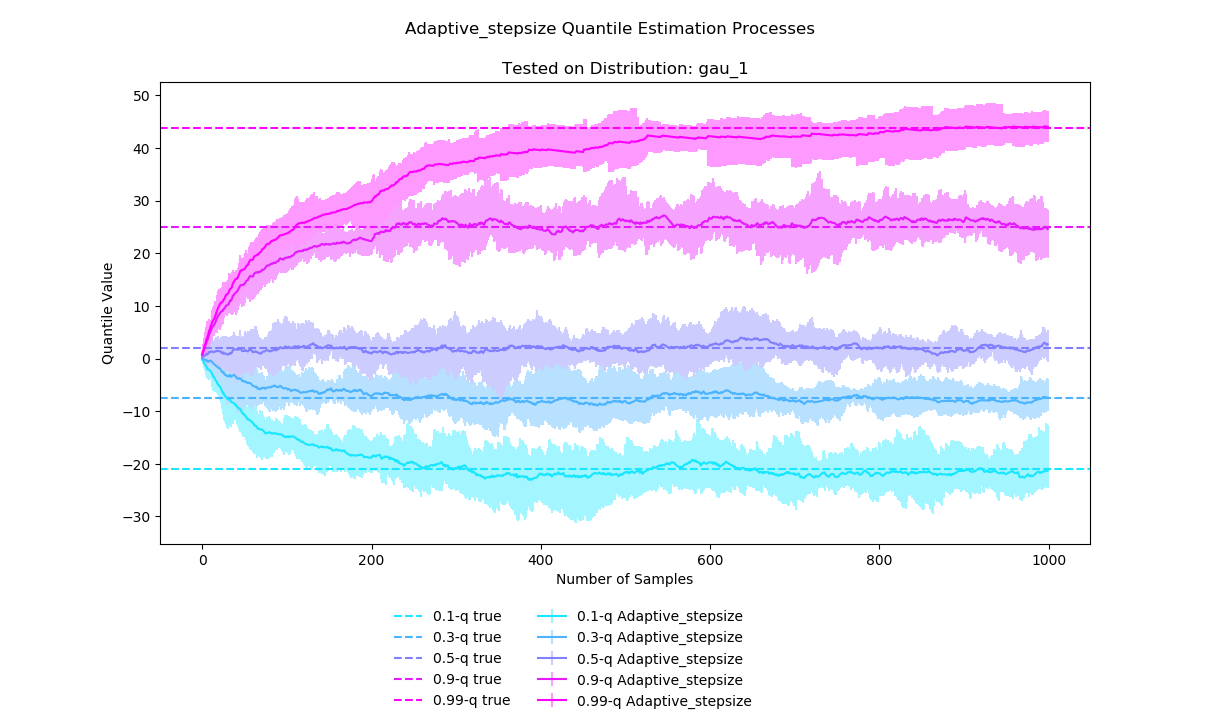
\includegraphics[width=1\columnwidth]{distro/gau_1_proc.png}
	\caption{DH-SGD Process from \textit{gau-1} Distribution}
\end{figure}

\begin{figure}[H]
    \centering
	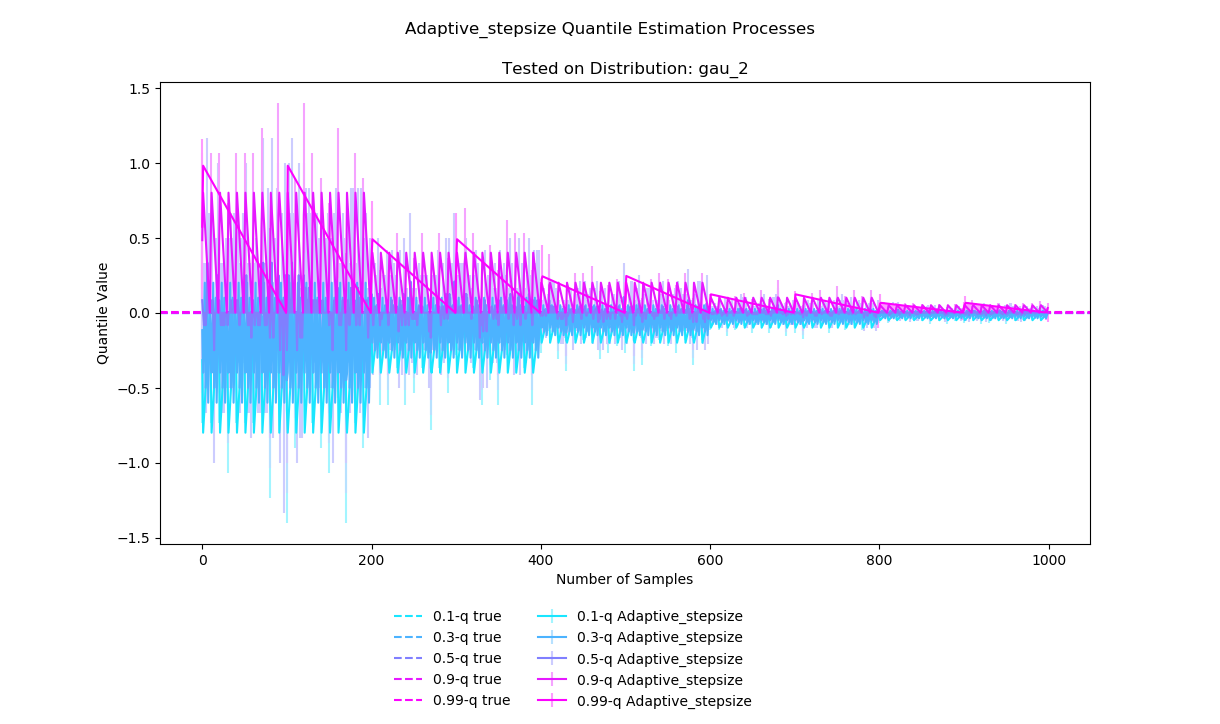
\includegraphics[width=1\columnwidth]{distro/gau_2_proc.png}
	\caption{DH-SGD Process from  \textit{gau-2} Distribution}
\end{figure}

\begin{figure}[H]
    \centering
	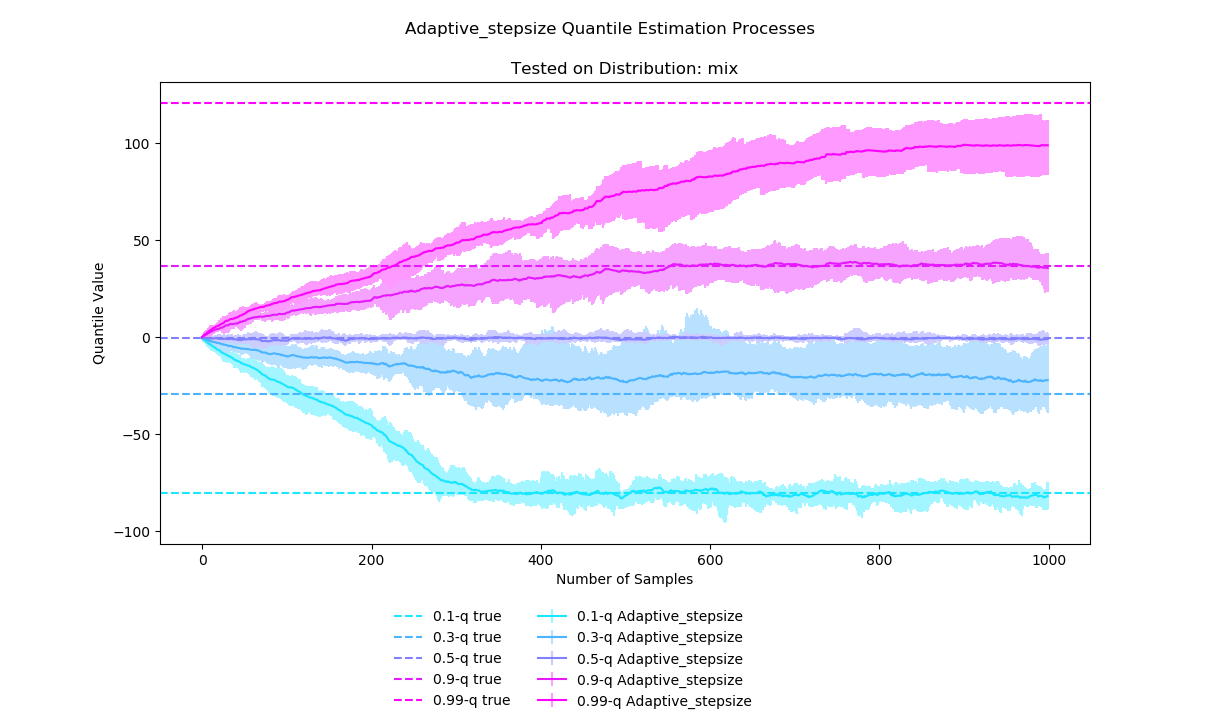
\includegraphics[width=1\columnwidth]{distro/mix_proc.png}
	\caption{DH-SGD Process from \textit{mix} Distribution}
\end{figure}

\begin{figure}[H]
    \centering
	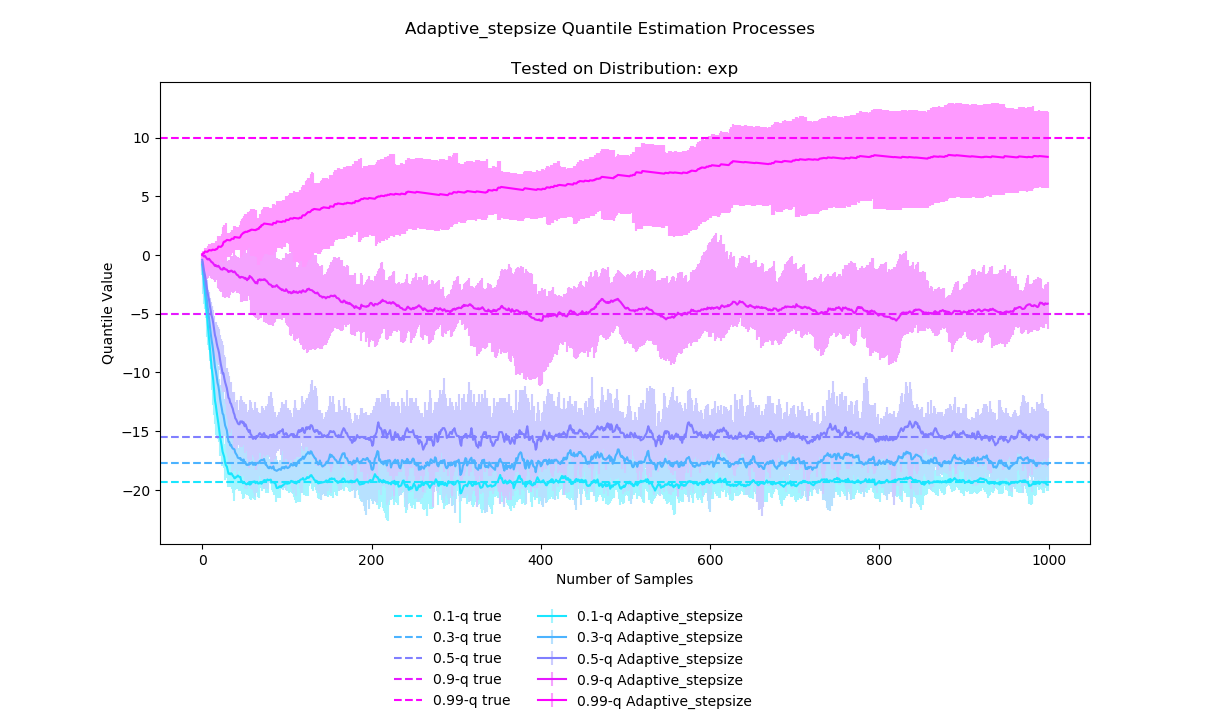
\includegraphics[width=1\columnwidth]{distro/exp_proc.png}
	\caption{DH-SGD Process from \textit{exp} Distribution}
\end{figure}

\begin{figure}[H]
    \centering
	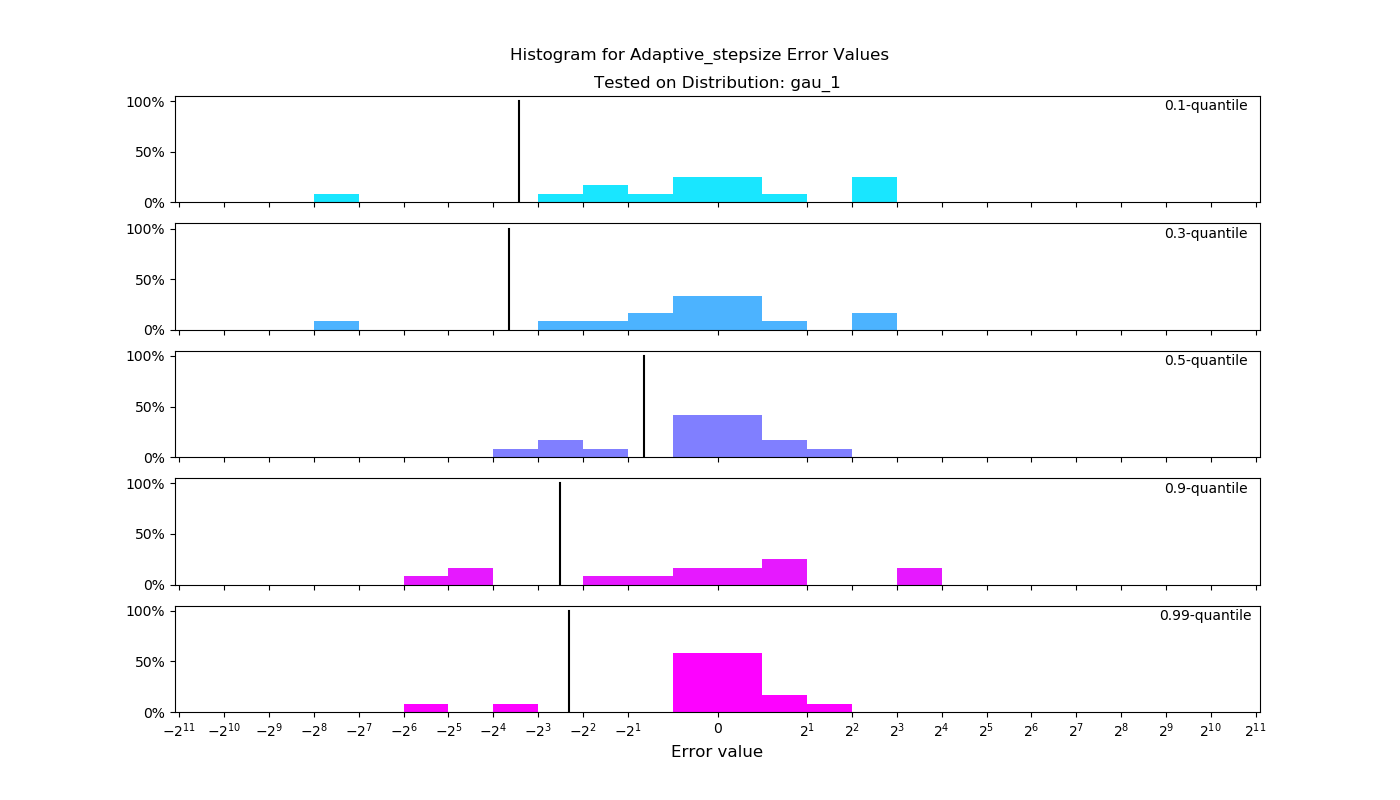
\includegraphics[width=1\columnwidth]{distro/gau_1_err.png}
	\caption{DH-SGD Error from \textit{gau-1} Distribution}
\end{figure}

\begin{figure}[H]
    \centering
	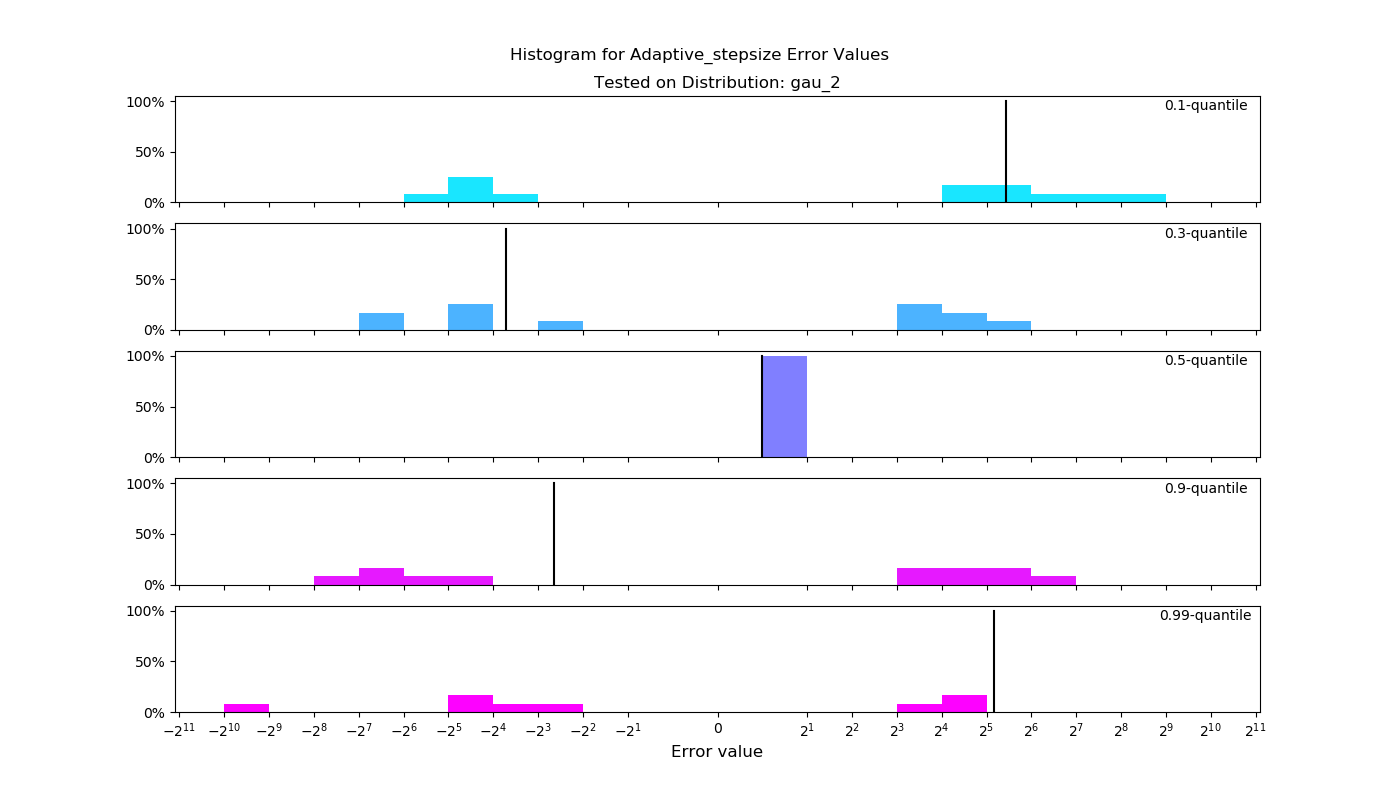
\includegraphics[width=1\columnwidth]{distro/gau_2_err.png}
	\caption{DH-SGD Error from  \textit{gau-2} Distribution}
\end{figure}

\begin{figure}[H]
    \centering
	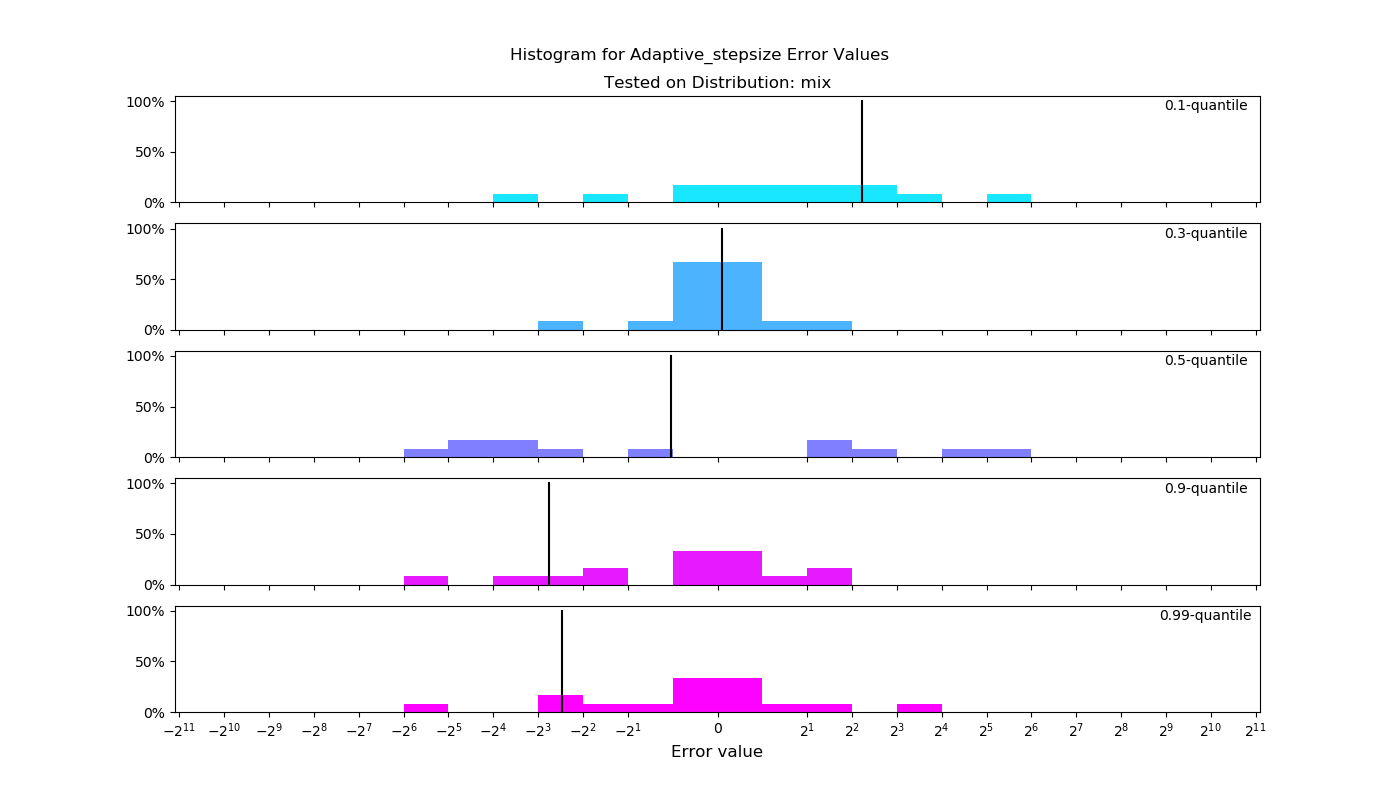
\includegraphics[width=1\columnwidth]{distro/mix_err.png}
	\caption{DH-SGD Error from \textit{mix} Distribution}
\end{figure}

\begin{figure}[H]
    \centering
	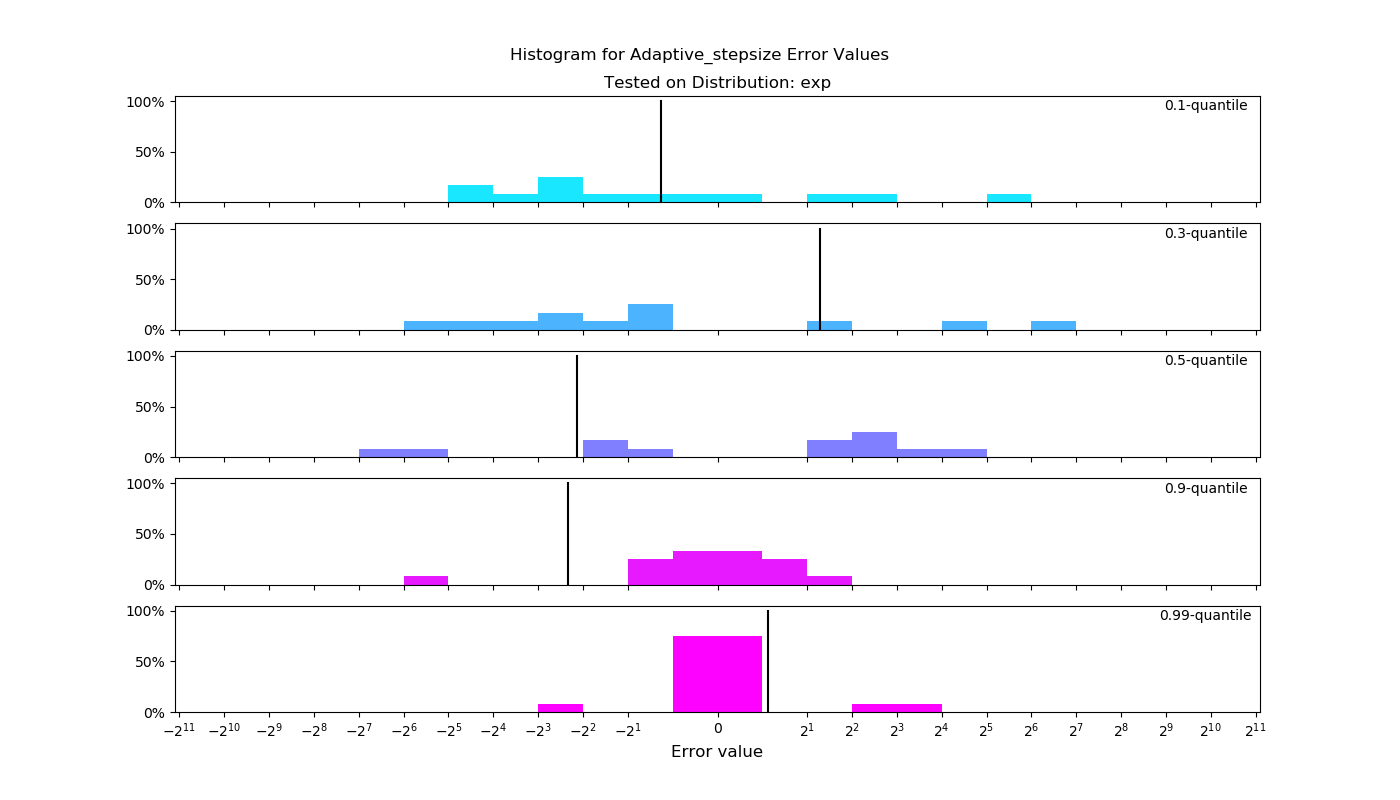
\includegraphics[width=1\columnwidth]{distro/exp_err.png}
	\caption{DH-SGD Error from \textit{exp} Distribution}
\end{figure}

\subsubsection{DH-SGD on Different Data Size}
\label{subsubsec: DH_SGD_exp_data_size}

\begin{figure}[H]
    \centering
	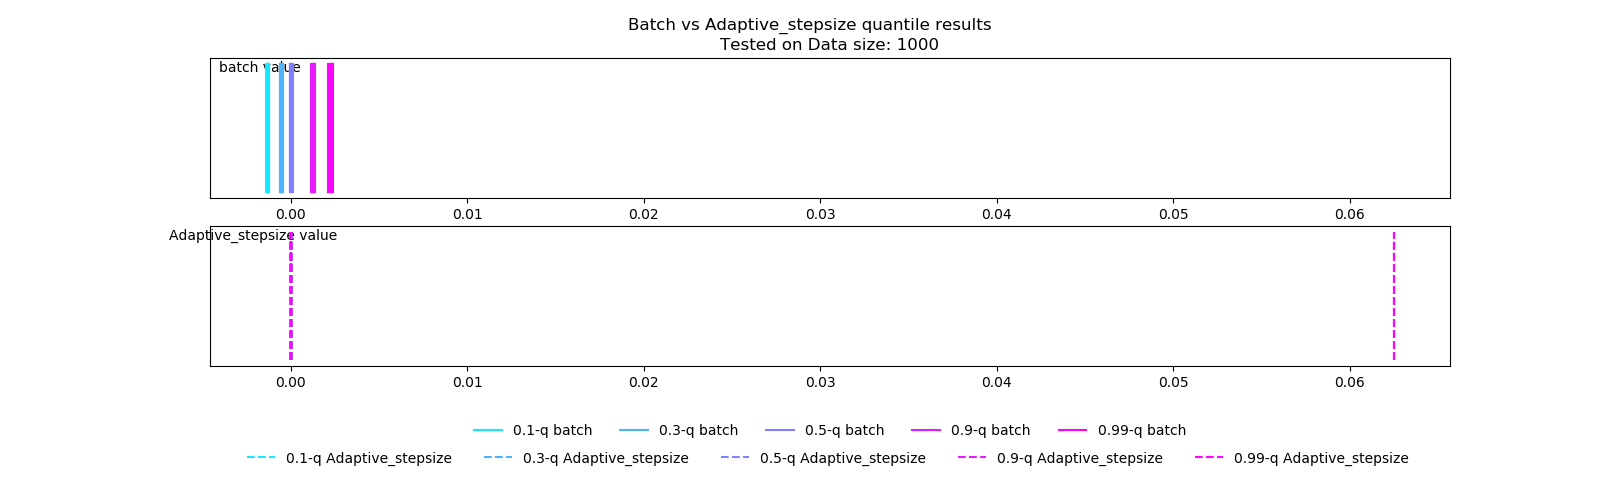
\includegraphics[width=1\columnwidth]{data_size/1000_res.png}
	\caption{DH-SGD Results from 1000 samples from \textit{gau-2} Distribution}
\end{figure}

\begin{figure}[H]
    \centering
	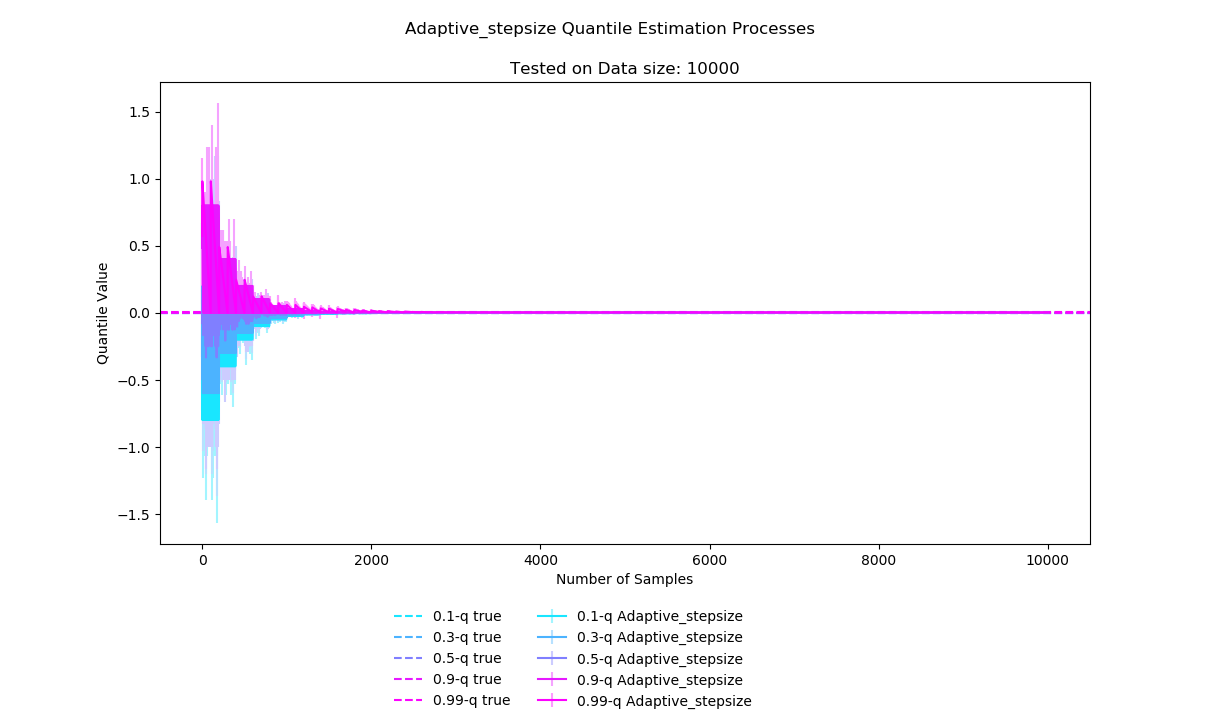
\includegraphics[width=1\columnwidth]{data_size/10000_proc.png}
	\caption{DH-SGD Process from 10000 samples from\textit{gau-2} Distribution}
\end{figure}

\begin{figure}[H]
    \centering
	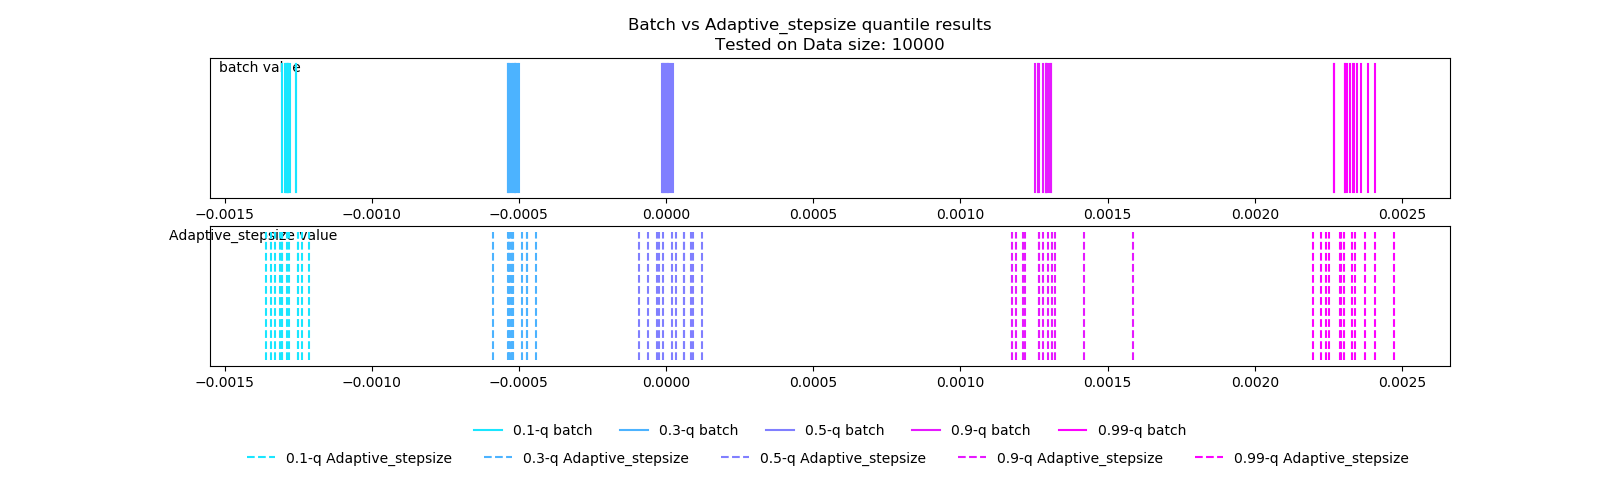
\includegraphics[width=1\columnwidth]{data_size/10000_res.png}
	\caption{DH-SGD Results from 10000 samples from \textit{gau-2} Distribution}
\end{figure}

\begin{figure}[H]
    \centering
	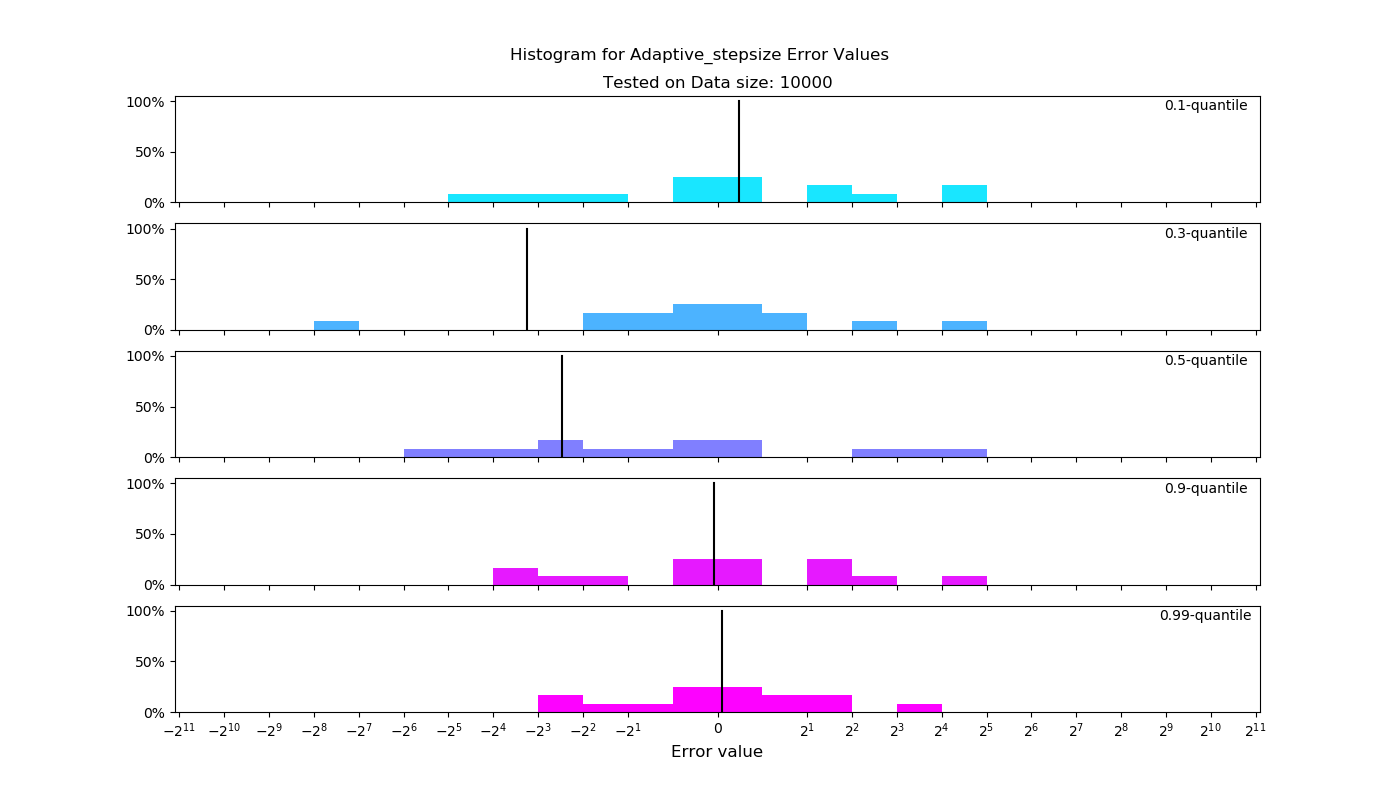
\includegraphics[width=1\columnwidth]{data_size/10000_err.png}
	\caption{DH-SGD Error from 10000 samples from \textit{gau-2} Distribution}
\end{figure}

\subsection{Discussion}

Choice on \textbf{step size check}:
    If step size check to be small: easier to have gau-2 converge within 1000 epochs, but not enough data for epoch checking
    If step size check large: the other way around
    Since we assume the data stream is big, maybe try with more than 200 epochs

    (try a different way) Can actually get easily solved by sorting the first F (F = 100 for example) quantiles and set the initialization and step size according to that

The judgement of\textbf{ "too small/big"} step size: 
    binomial distro for different quantiles The possibility that there are exactly $x$ epochs  going up in the total of $n$ epochs for $\tau$ when the quantile has converged.
    The distribution is different for different $\tau$ and different $n$, but $n$ does not matter that much as $\tau$ in this situation. It means the distance between of \textbf{dfa} should be different for different $\tau$.


\section{Discussion and conclusion}

Compare SAG, Doubling-and-Halving SGD and SGD

Conclusion: both are good methods lol

1. Convergence rate:

2. Fluctuation after convergence

5. Further improvement: SAG + DH SGD?
